% ---
% primeiro capitulo de Resultados
% ---
\chapter{Resultados}

Neste capítulo, os resultados e a análise dos experimentos realizados durante o trabalho são reportados. Os resultados obtidos nos testes de validação apresentam a média dos valores coletados após diversas execuções dos cenários de forma sequencial.

Foram executadas 30 interações para cada requisição necessária a fim de obeter as respostas das questões levandas no capítulo anterior. Os dados necessários puderam ser buscados em uma única requisição à API GraphQL, enquanto foram precisos à API REST duas requisições para chegar a resposta da primeira questão, e vinte e oito para obter a resposta da segunda. Os detalhes podem ser constatados nas tabelas \ref{tab:request-table1} e \ref{tab:request-table2}.

\begin{table}[htbp]
    \centering
    \begin{tabular}{| l | l | l |}
        \hline
        \textbf{Requisição} & \textbf{Resultado} & \textbf{Número de requisições} \\ \hline
        /pallets & Todos os pallets & 1x \\ \hline
        /items/:id & Detalhes do item mais presente & 1x \\ \hline
    \end{tabular}
    \caption{Fluxo de dados para responder Questão 1} 
    \label{tab:request-table1}
\end{table}

\begin{table}[htbp]
    \centering
    \begin{tabular}{| l | l | l |}
        \hline
        \textbf{Requisição} & \textbf{Resultado} & \textbf{Número de requisições} \\ \hline
        /items & ID do item 22B12 & 1x \\ \hline
        /items/:id & Detalhes do item 22B12 & 1x \\ \hline
        /pallets & Pallets contendo item 22B12 & 1x \\ \hline
        /pallets/:id & Detalhes do Pallet contendo o item 22B12 & 5x \\ \hline
        /addresses/:id & Detalhes do Endereço contendo o item 22B12 & 5x \\ \hline
        /levels/:id & Nível contendo o item 22B12 & 5x \\ \hline
        /slots/:id & Prateleira contendo o item 22B12 & 5x  \\ \hline
        /rows/:id & Linha contendo o item 22B12 & 5x \\ \hline
    \end{tabular}
    \caption{Fluxo de dados para responder Questão 2} 
    \label{tab:request-table2}
\end{table}

Alem das 30 interações feitas para cada requisição, foi montado também tres cenários para melhor analise dos resultados. Estes cenáios possuem quantidade de registros diferentes para as entidades Item e Pallet, pois são estas que afetam de maneira mais significativa o quão eficiente será a resposta das APIs. Estes tres cenários estão descritos na tabela \ref{tab:cenarios} com suas respectivas quantidades.

\begin{table}[htbp]
    \centering
    \begin{tabular}{| l | l | l | l|}
        \hline
        \textbf{Recurso} & \textbf{C1} & \textbf{C2} & \textbf{C3} \\ \hline
        Item & 1000 & 10000 & 30000 \\ \hline
        Pallet & 1000 & 10000 & 30000 \\ \hline
        Address & 156 & 156 & 156 \\ \hline
        Slot & 26 & 26 & 26 \\ \hline
        Row & 2 & 2 & 2 \\ \hline
        Level & 3 & 3 & 3 \\ \hline
    \end{tabular}
    \caption{Cenários analisados} 
    \label{tab:cenarios}
\end{table}

\section{Questão 1}

Embora necessite de buscas mais simples, através da Questão 1 já é possível observar as diferenças em termos de desempenho entre aplicaçãoes REST e aplicaçãoes GraphQL. A Questão 1 busca o Item que ocupa a maior quantidade de pallets alocados no armazém, e para responde-la é necessário fazer duas requisições. A primeira busca todos os pallets registrados nas APIs, e após identificado qual o item mais comum presente nos \textit{Pallets} registrados, a segunda requisição busca os detalhes deste.

\subsection{Utilização da CPU}

Ao analisarmos a utilização da CPU, ilustrado na figura \ref{fig:q1-cpu}, percebemos que as APIs REST e GraphQL tem desempenho similares com consultas de C1 e C2. Por outro lado, as consultas de C3, mostram a API REST muito menos eficiente ao utilizar a CPU.

\begin{figure}[htbp]
    \centering
    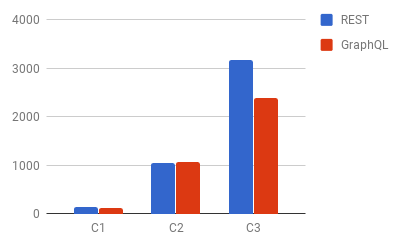
\includegraphics[width=0.8\textwidth]{figuras/q1-cpu.png}
    \caption{Comparação da Utilização de CPU}
    \label{fig:q1-cpu}
    \author{fonte: Autor}
\end{figure}

As consultas de C1 exigiram 133.8 ms de CPU na API REST e apenas 111.10 ms na API GraphQL. executando C2 a API REST consumiu 1042.52 ms na CPU enquanto a API GraphQL consumiu 1065.45 ms, e é neste cenário que notamos a maior similaridade entre as APIs no consumo da CPU. Por outro lado, quando quando analisado os resultados de C3, nota-se uma grande desvantagem para API REST, que utilizou 3177.6 ms da CPU enquanto a API GraphQL usou apenas 2382.1 ms.
    
\subsection{Consumo de memória}

Os dados do resultado da comparação do consumo de memória expõem que a API REST também se mostrou menos eficiente neste quesito em relação a API GraphQL. Os resultados podem ser obervados na figura \ref{fig:q1-mem}

\begin{figure}[htbp]
    \centering
    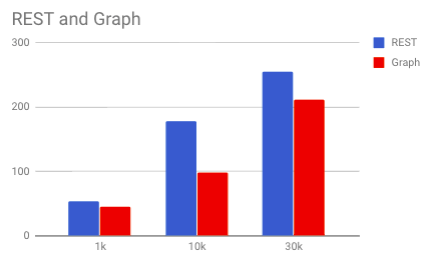
\includegraphics[width=0.8\textwidth]{figuras/q1-mem.png}
    \caption{Comparação do Consumo de Memória}
    \label{fig:q1-mem}
    \author{fonte: Autor}
\end{figure}

Ao compararmos os resultados de C1 e C3, a API REST se mostrou cerca de 20\% menos eficiente que a API GraphQL. O que se destaca é quando comparamos os resultados de C3, em que a API GraphQL consumiu 127.71 megabytes de memória e a API REST consumiu 178.01 megabytes, uma diferença de quase 40\%.

\subsection{Tempo de resposta}

Como esperado, a API implementada com GraphQL realmente respondeu as consultas em um tempo menor do que a API REST. A figura \ref{fig:q1-time} mostra a diferença do tempo de respota das APIs para executar as consultas da primeira questão.

\begin{figure}[htbp]
    \centering
    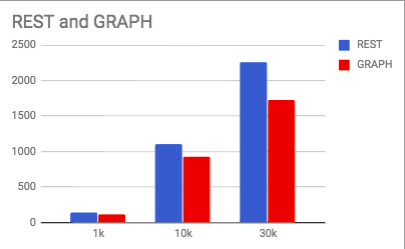
\includegraphics[width=0.8\textwidth]{figuras/Q1-result-request-time.png}
    \caption{Comparação do tempo de resposta}
    \label{fig:q1-time}
    \author{fonte: Autor}
\end{figure}

Nas requisições de C1, a API REST teve como resultado um tempo de resposta de 147.3 ms, enquanto a API GraphQL respondeu a consulta em 115.63 ms, representando uma diferença de X por cento. Ao analizar as consultas de C2, a API REST respondeu as consultas em 1108.13 ms e a API GraphQL devolveu os resultados em 925.63 ms, uma diferença de Y por cento. Por último, as consultas de C3 foram respondidas em 2261.1 ms na API REST e 1725.7 ms na API GraphQL, o que representa uma diferença de Z por cento.

\subsection{Tamanho da resposta}

Outro resultado esperado era que o tamanho da resposta da API GraphQL fosse menor do que o tamanho da resposta da API REST. Essa hipótese se confirmou como pode ser visto da figura \ref{fig:q1-size}.

\begin{figure}[htbp]
    \centering
    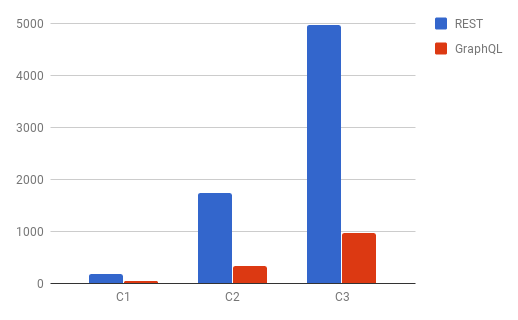
\includegraphics[width=0.8\textwidth]{figuras/Q1-size.png}
    \caption{Comparação do tamanho de resposta}
    \label{fig:q1-size}
    \author{fonte: Autor}
\end{figure}

A API REST respondeu as requisições da questão 1 com um tamanho de resposta de 174.04 Kb, 1740.17 Kb e 4980 Kb para C1, C2, C3 respectivamente. Da mesma maneira, a API GraphQL teve como resultado respostas com 31.68 Kb, 322.53Kb e 967.35Kb. 

%%--------------
%%--------------
%%--------------

\section{Questão 2}

Para as repostas da questão 2, as consultas foram mais complexas na API GraphQL, e mais numerosas na API REST. 

\subsection{Utilização da CPU}

Analisando os resultados da utilização de CPU, podemos concluir que a API GraphQL utiliza desse recurso de uma maneira mais eficiente do que a API REST. A figura \ref{fig:q2-cpu} ilustra os resultados obtidos comparando o uso da CPU.

\begin{figure}[htbp]
    \centering
    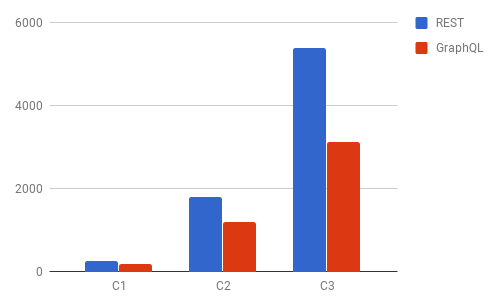
\includegraphics[width=0.8\textwidth]{figuras/q2-cpu.png}
    \caption{Comparação da Utilização da CPU - Q2}
    \label{fig:q2-cpu}
    \author{fonte: Autor}
\end{figure}

Aqui a diferença nos resultados obtidos é notada com mais clareza a medida em que aumentamos o número de registros. Analizando C1, a API REST exiigu 244.41 ms da CPU para ser processada, ao mesmo tempo que a API GraphQL exigiu somente 178.22 ms. Nas consultas de C2, a API REST demandou 1787.74 ms para ser processada, e a API GraphQL demandou 1199.53 ms. A maior diferença encontra-se em C3, onde a API REST levou 5383.40 ms para ser completamente processada pela CPU e a API GraphQL levou apenas 3132.98 ms.

\subsection{Consumo de memória}

Os dados referentes ao consumo de memória estão ilustrados na figura \ref{fig:q2-mem}, e apontam que a API REST faz uso menos eficiente deste recurso, comparando com o consumo de memória da API GraphQL. Foi analisando esta métrica que se encontrou o único cenário onde a API REST se mostrou mais eficiente que a API GraphQL.

\begin{figure}[htbp]
    \centering
    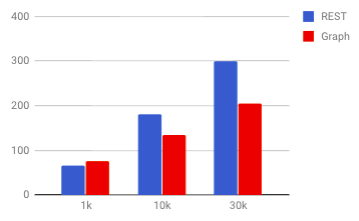
\includegraphics[width=0.8\textwidth]{figuras/q2-mem.png}
    \caption{Comparação do Consumo de memória Q2}
    \label{fig:q2-mem}
    \author{fonte: Autor}
\end{figure}

O consumo de memória não se mostrou tão diferentes comparando as APIs. Nas requisições de C1, a API REST demonstra ser mais eficiente, mesmo que a diferença seja de apenas 9.88 megabytes, em relação a API GraphQL. A API GraphQL consumiu 76.19 mb de memória, contra 66.27 consumidos pela API REST. Essa melhor eficiencia já não é mais identificada em C2, onde a API REST consumiu 181.02 mb de meória, e a API GraphQL consumiu 133.52 mb. Nas consultas de C3, observamos uma diferença relevante no consumo de mémoria, com a API REST consumindo 300.30 mb de memória enquanto a API GraphQL consumindo 206.02, uma impressionante diferença de quase 100 mb.

\subsection{Tempo de resposta}

Como mostra a figura \ref{fig:q2-time}, é possivel identificar com clareza que a API REST leva um tempo consideravelmente maior para responder todas as requisições comparando com o tempo levado pelas consultas na API GraphQL.

\begin{figure}[htbp]
    \centering
    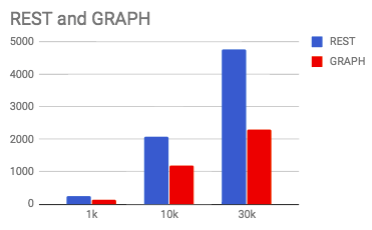
\includegraphics[width=0.8\textwidth]{figuras/Q2-result-request-time.png}
    \caption{Comparação do tempo de resposta Q@}
    \label{fig:q2-time}
    \author{fonte: Autor}
\end{figure}

Considerando as consultas de C1, a API REST teve como resultado um tempo de resposta de 254.56 ms, enquanto a API GraphQL respondeu a consulta em 148.5 ms, representando uma diferença de X por cento. Quando analisado as requisições de C2, a API REST respondeu as consultas em 2072.03 ms e a API GraphQL devolveu o resultado em 1201.3 ms, uma diferença de Y por cento. Por último, as consultas de C3 foram respondidas em 4770.2 ms na API REST e 2291.1 ms na API GraphQL, o que representa uma diferença de Z por cento.

\subsection{Tamanho da resposta}

A API GraphQL também mostrou-se mais vantajosa em termos de tamanho da resposta na Questão 2. A figura \ref{fig:q2-size} mostra a comparação entre os protótipos quando comparados esta métrica.

\begin{figure}[htbp]
    \centering
    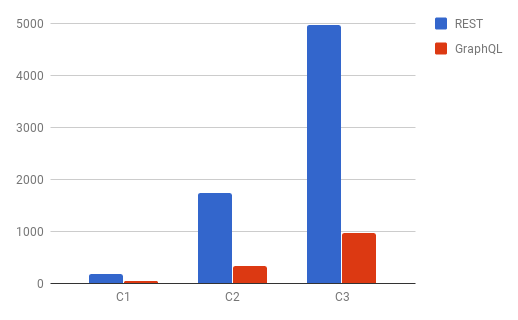
\includegraphics[width=0.8\textwidth]{figuras/Q1-size.png}
    \caption{Comparação do tamanho da resposta}
    \label{fig:q2-size}
    \author{fonte: Autor}
\end{figure}

A API REST respondeu as requisições da questão 1 com um tamanho de resposta de 259.53 Kb, 2522.17 Kb e 7221 Kb para C1, C2 e C3 respectivamente. Da mesma maneira, a API GraphQL teve como resultado respostas com 101.73 Kb, 1005.23 Kb e 2850 Kb. 

    